\documentclass{beamer}

\mode<presentation>
{
\usetheme{Darmstadt}

\setbeamercovered{transparent}
\useoutertheme{smoothbars}
}
\addtobeamertemplate{footline}{\insertframenumber/\inserttotalframenumber}

\usepackage[utf8]{inputenc} \usepackage[english]{babel}
\usepackage{graphicx} \usepackage{geometry}
\usepackage{pifont}
\usepackage{hyperref}
\usepackage{xspace}
\usepackage{fancyvrb}
\DefineVerbatimEnvironment{verbatim}{Verbatim}{formatcom=\color{blue}}


\newcommand{\E}[1]{{\textbf{#1}}}
\newcommand{\C}[1]{{\color{red}\texttt{#1}}}
\definecolor{mygreen}{cmyk}{0.888,0,0.888,0.298}
\newcommand{\G}[1]{{\color{mygreen}{#1}}}
% \newcommand{\B}[1]{{\color{blue}{#1}}}
% \newcommand{\ar}{\ding{220} }
% \newcommand{\todo}[1]{{\colorbox{yellow}{\color{fg}#1}}}
\newcommand{\eg}{\textit{e.g.}\xspace}
\newcommand{\gridk}{{Grid'5000}\xspace}
% \newcommand{\execo}{\textsc{Execo}\xspace}
% \newcommand{\myvspace}{\vspace{0.5em}}

\title{Kwapi for Grid'5000}
\subtitle{A distributed infrastructure for large scale power measurements}

\author[LIP Team]{Laurent Pouilloux \and François Rossigneux \and Laurent
Lefèbvre \and Simon Delamare}
\institute[INRIA/LIP ENS-Lyon]{INRIA/LIP ENS-Lyon}
\date{27/03/2014}

% Delete this, if you do not want the table of contents to pop up at
% the beginning of each subsection:
\AtBeginSection[]
{
\begin{frame}<beamer>
\frametitle{Outline}
\tableofcontents[currentsection,currentsubsection,hideothersubsections]
\end{frame}
}

\begin{document}
\begin{frame}
\titlepage
\end{frame}
% \maketitle
%
% \frame{\tableofcontents}
%
\section*{Introduction}

\begin{frame}{Contexte}
\begin{itemize}
  \item Consommation mondiale des datacenters augmente à fond avec l'explosion
  du cloud
  \item Pose un problème pour le futur avec l'exascale et \ldots
  \item Augmenter le flops/Watt
  \item besoin d'expérimenter sur Grid'5000
  \begin{itemize}
    \item matériel
    \item applicative
    \item système
  \end{itemize}
\end{itemize}

\alert{Besoin d'une infrastructure de monitoring énergétique, distribuée sur
les sites et à haute résolution}
\end{frame}


\section{Fonctionnalités}

\begin{frame}{Les mesures actuelles}
api\_pdu.py pour générer le tableau actuel
\end{frame}

\begin{frame}{Outils existants pour récupérer les données}

\begin{block}{API}

\end{block}

\begin{exampleblock}{wattmetre.lyon.grid5000.fr}
\begin{minipage}{0.77\linewidth}
\begin{itemize}
  \item Wattmetre Omega 3
  \item Visualisation ``temps réelle'' des mesures
  \item Récupération des logs des machines
\end{itemize}
\end{minipage}
\hfill
\begin{minipage}{0.17\linewidth}
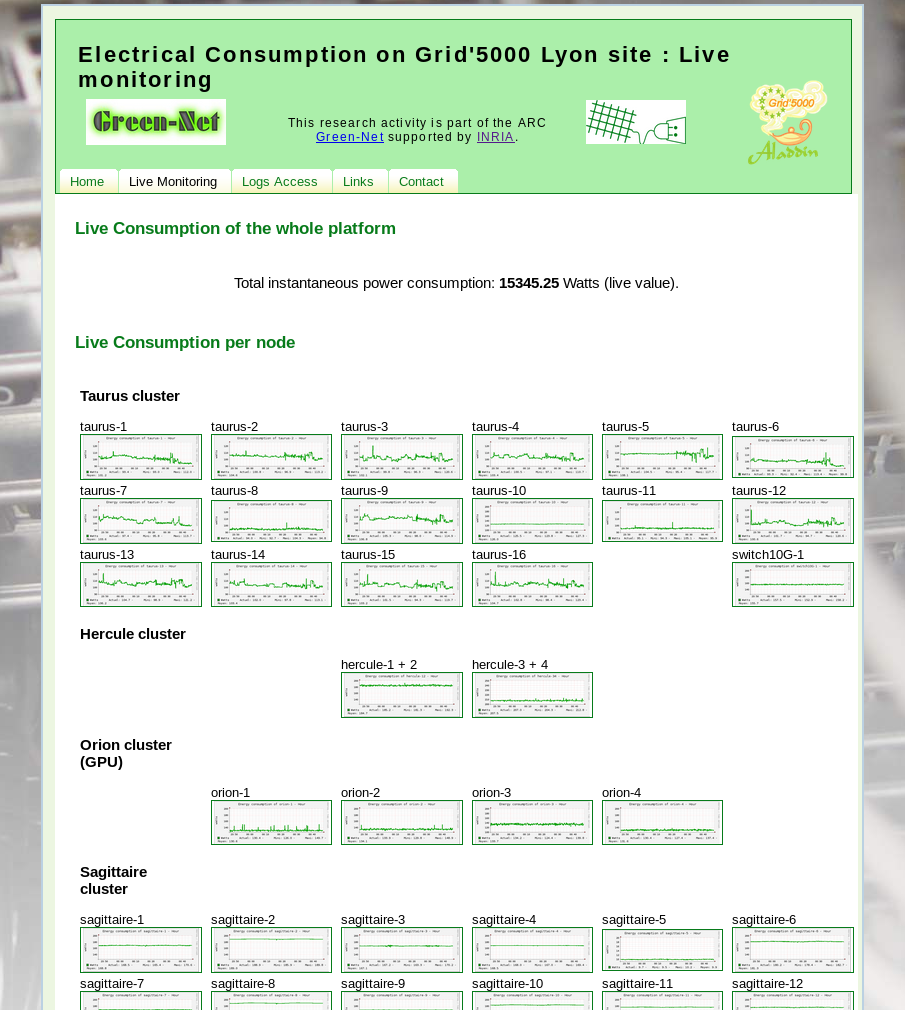
\includegraphics[width=\linewidth]{live_monitoring.png}
\end{minipage}
\end{exampleblock}

\end{frame}

\begin{frame}{Que veut-on ?}
\begin{itemize}
  \item uniformiser l'infra de monitoring
  \item remplacer les scripts qui mettent à jour ganglia
  \item fournir aux utilisateurs les données de mesures précises pendant 1 an
  \item permettre une visualisation live des expériences
\end{itemize}
\end{frame}



\section{Architecture}

\begin{frame}{Vue générale}
\begin{minipage}{0.47\linewidth}
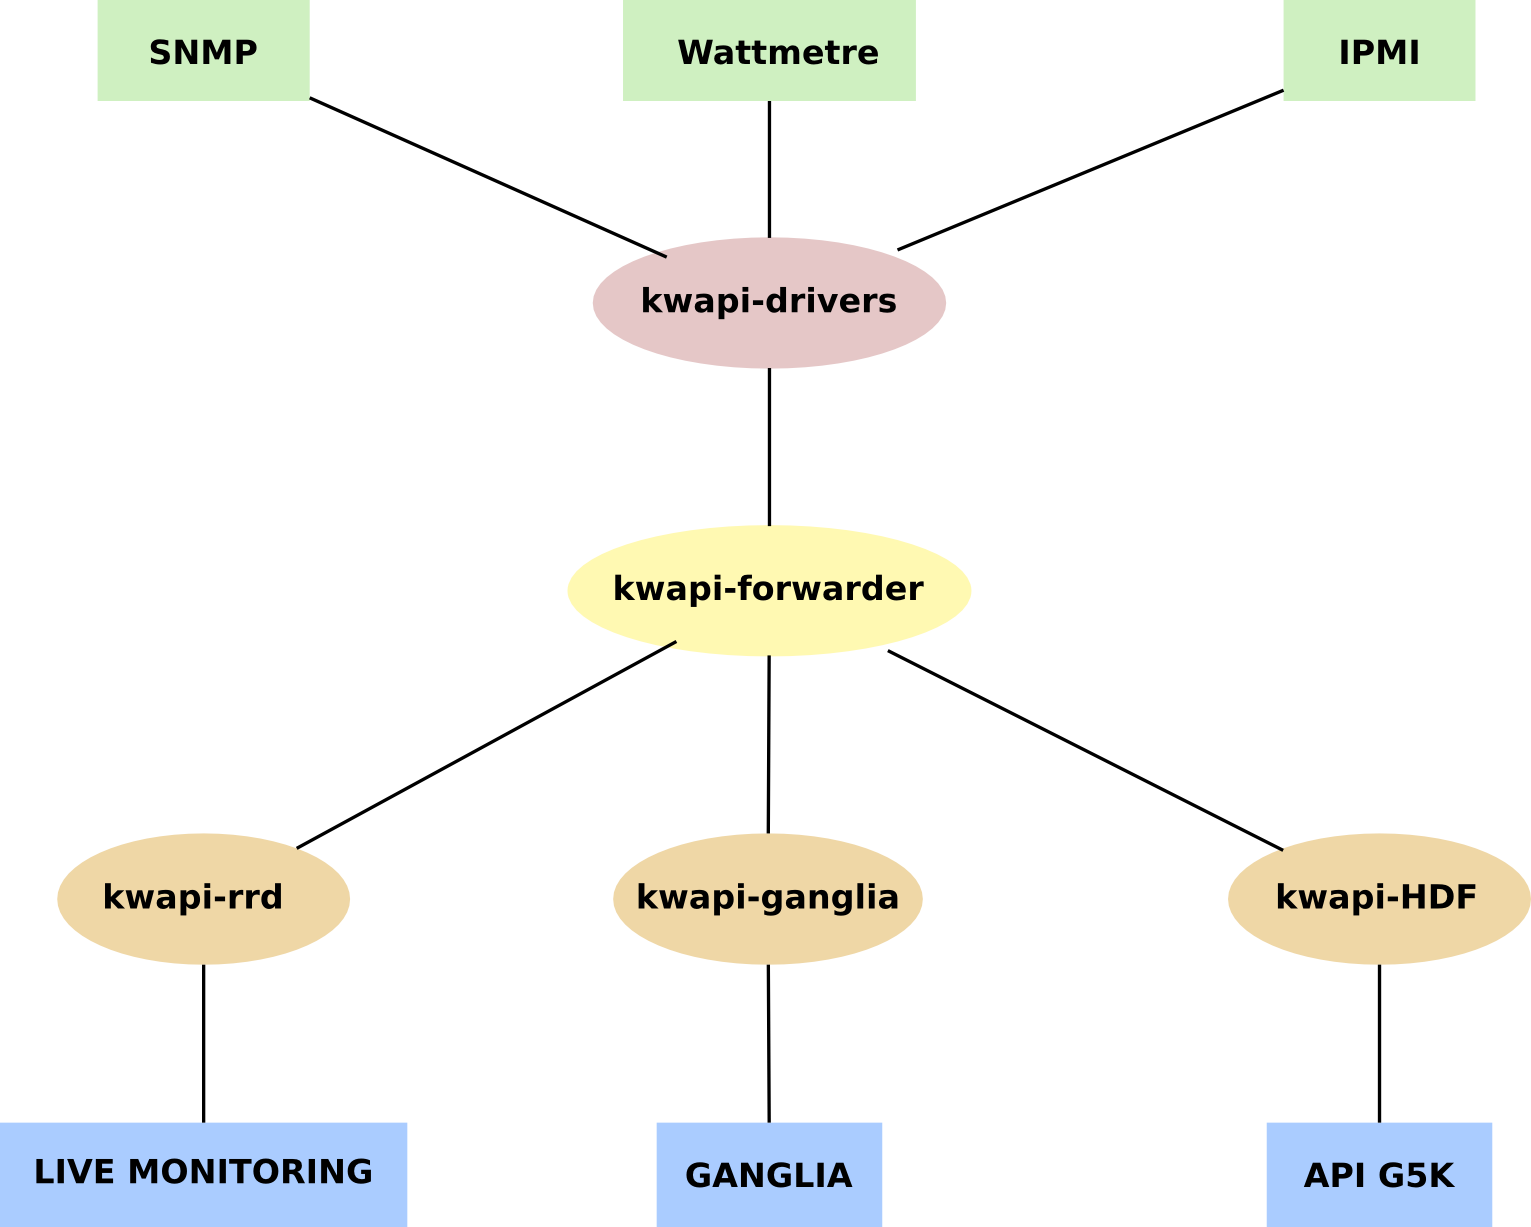
\includegraphics[width=\linewidth]{Kwapi_archi.png}
\end{minipage}
\hfill
\begin{minipage}{0.47\linewidth}
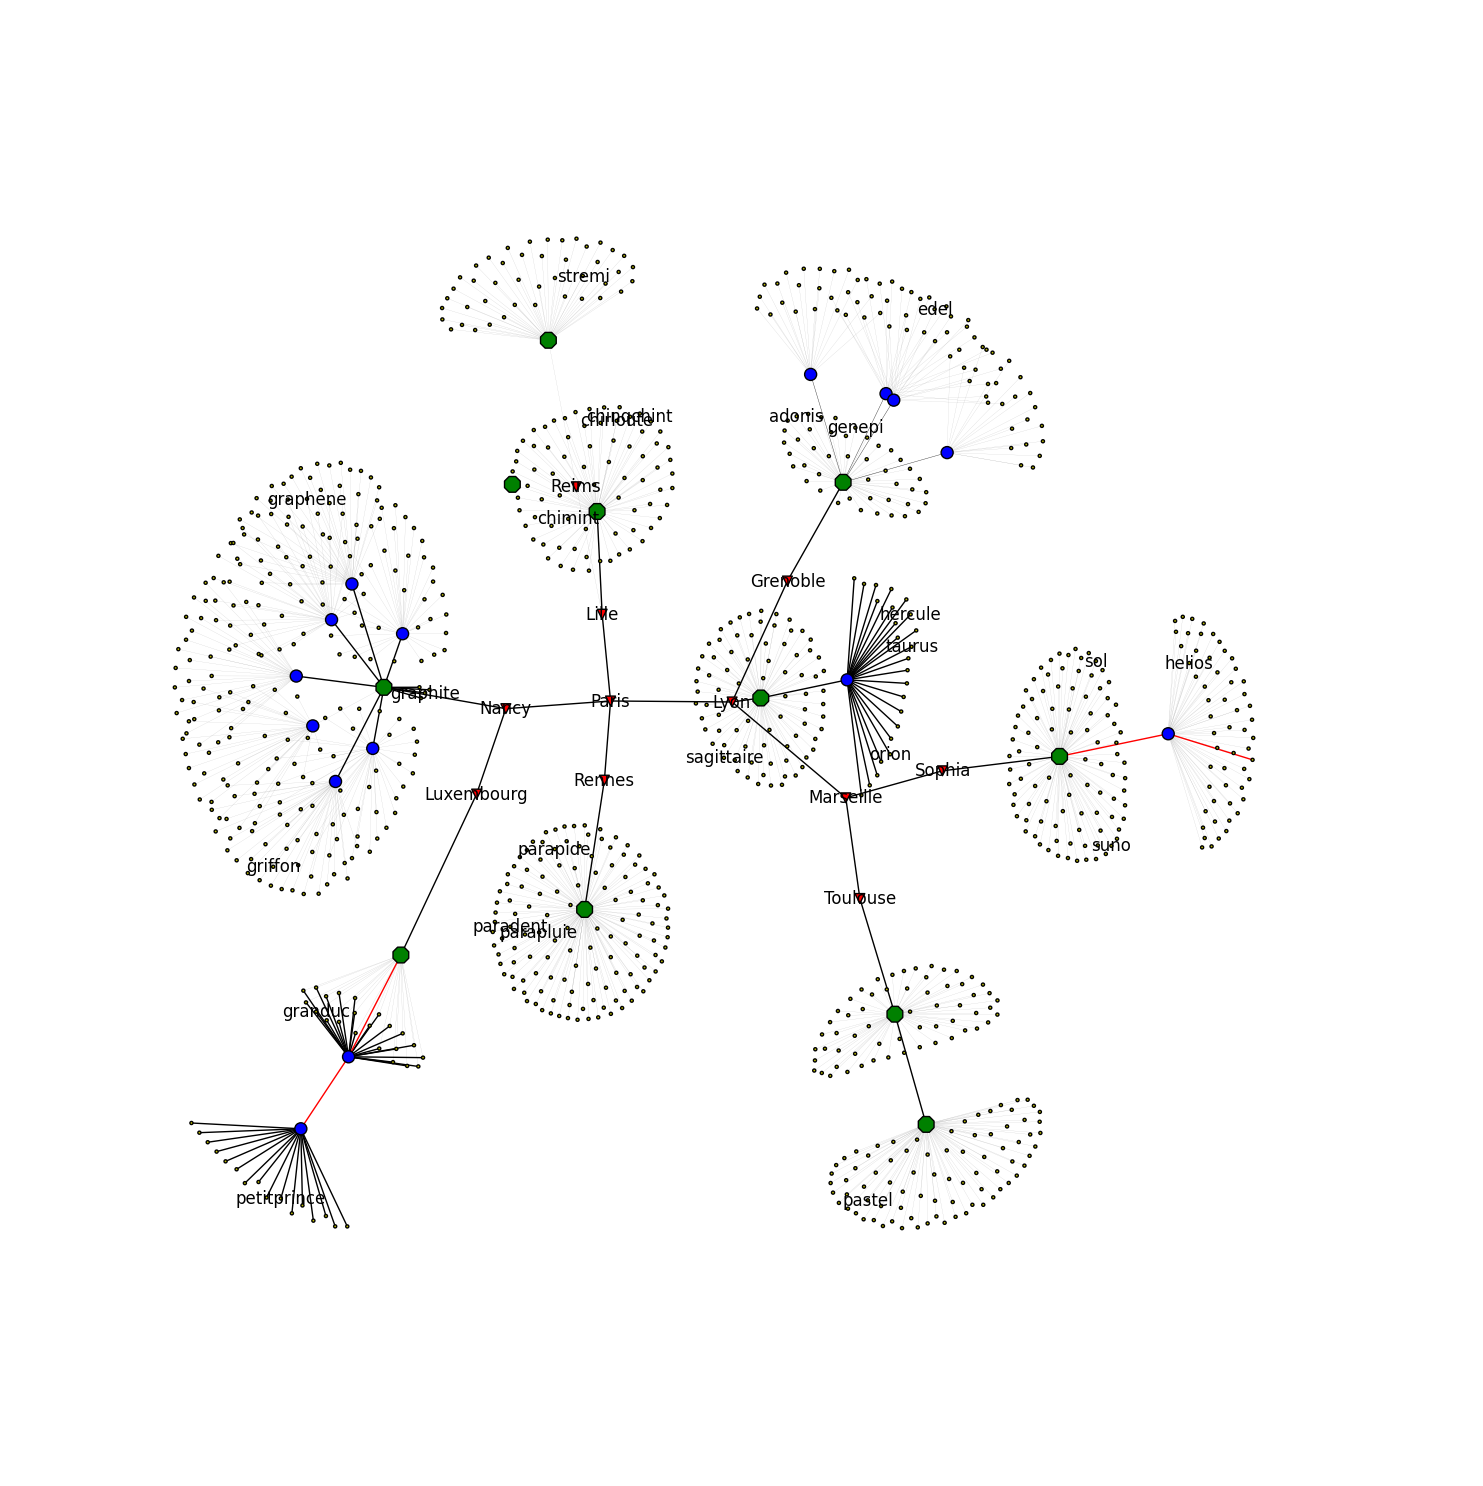
\includegraphics[width=\linewidth]{topo5k.png}
\end{minipage}
\end{frame}

\begin{frame}{Besoins}
\begin{itemize}
  \item une VM par site
  \item 100 To par an
\end{itemize}

Information dans l'API Grid'5000
\end{frame}

\begin{frame}{Récupération des données sur les équipements}

\begin{itemize}
  \item Driver manager
  \item Forwarder
\end{itemize}
\end{frame}

\begin{frame}{Visualisation temps-réelle}

\end{frame}


\begin{frame}{Données haute résolution}

\end{frame}

\begin{frame}{Mise à jour de Ganglia}

\end{frame}

\begin{frame}{Intégration dans l'API Grid'5000}

\end{frame}



\section{Tests}

\begin{frame}{Comparatif Ganglia-Live}
à faire
\end{frame}

\begin{frame}{Procédure d'installation}
Maxime à Grenoble ?
Hyacynthe à Luxembroug
\end{frame}



\begin{frame}{Jenkins}
\begin{itemize}
  \item Vérification automatique des données de l'API
\end{itemize}
\end{frame}


\section*{Conclusion}

\begin{frame}{Bilan}

\end{frame}

\begin{frame}{La suite}


\end{frame}




\end{document}